\documentclass{article}
\usepackage[utf8]{inputenc}
\usepackage{enumerate}
\usepackage{enumitem}
\usepackage{float}
\usepackage{graphicx}
\usepackage{multirow, array}


\title{Práctica 2: Gestión de una Web de cine}
\author{Rafael Nogales Vaquero
\\Lothar Soto Palma
\\Elena Toro Pérez
\\Jose Ramón Trillo Vilchez}
\date{5 Noviembre del 2014}

\begin{document}

\maketitle

\section{Introducción}
\section{Jerarquia de casos de uso}
\subsection*{Gestión de Usuarios}
	\begin{description}
	\item[Descripción]:\\ Escenarios asociados con la gestión de usuarios,clientes y administradores/empleados.
	\item[Casos de Uso]:\\ Registro(Alta usuario), Consultar películas, Modificar información de usuario, Consultar información de Usuario, Consultar cuenta de Usuario, Votar Películas, Comentar/criticar Películas, Eliminar cuenta de Usuario, Acceder a lista de Almas Gemelas, Comprar Película, Comprar Película, Consulta a Empleado/Administrador, Identificar Usuario, Método de pago, Actualizar Películas, Añadir/borrar Películas, Control de comentarios/críticas, Moderación de usuarios, Listar usuarios Baneados del sistema, Listar usuarios colaboradores, Banear usuarios.
	\item[Actores]:\\ Cliente, Usuario, Administrador, Sistema.
	\end{description}
\subsection*{Gestión de Almas Gemelas}
\subsection*{Gestión de Películas}
\subsection*{Gestión de Ventas}
	\begin{description}
	\item[Descripción]:\\ Escenarios asociados con la gestión de ventas de películas.
	\item[Casos de Uso]:\\ Comprar Película, Reservar Película, Identificar Socio, Disponibilidad de Películas, Pago a Cuenta, Pago en Metálico, Pago con Tarjeta.
	\item[Actores]:\\ Usuario, Administrador.
	\end{description}
\section{Diagrama de paquetes}
	\begin{center}
   		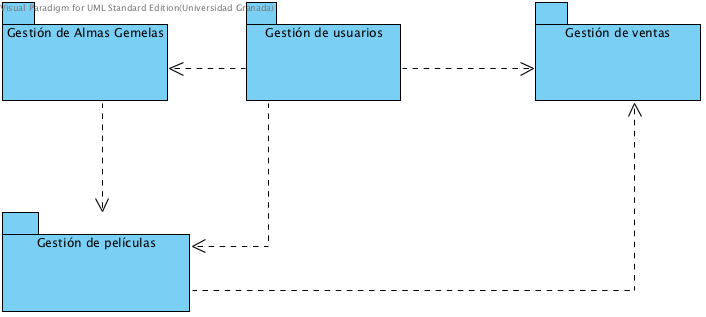
\includegraphics[scale=0.75]{Paquetes.png}
   	\end{center}

\section{Diagrama de casos de uso}
\subsection*{Gestión de Usuarios}
	\begin{center}
   		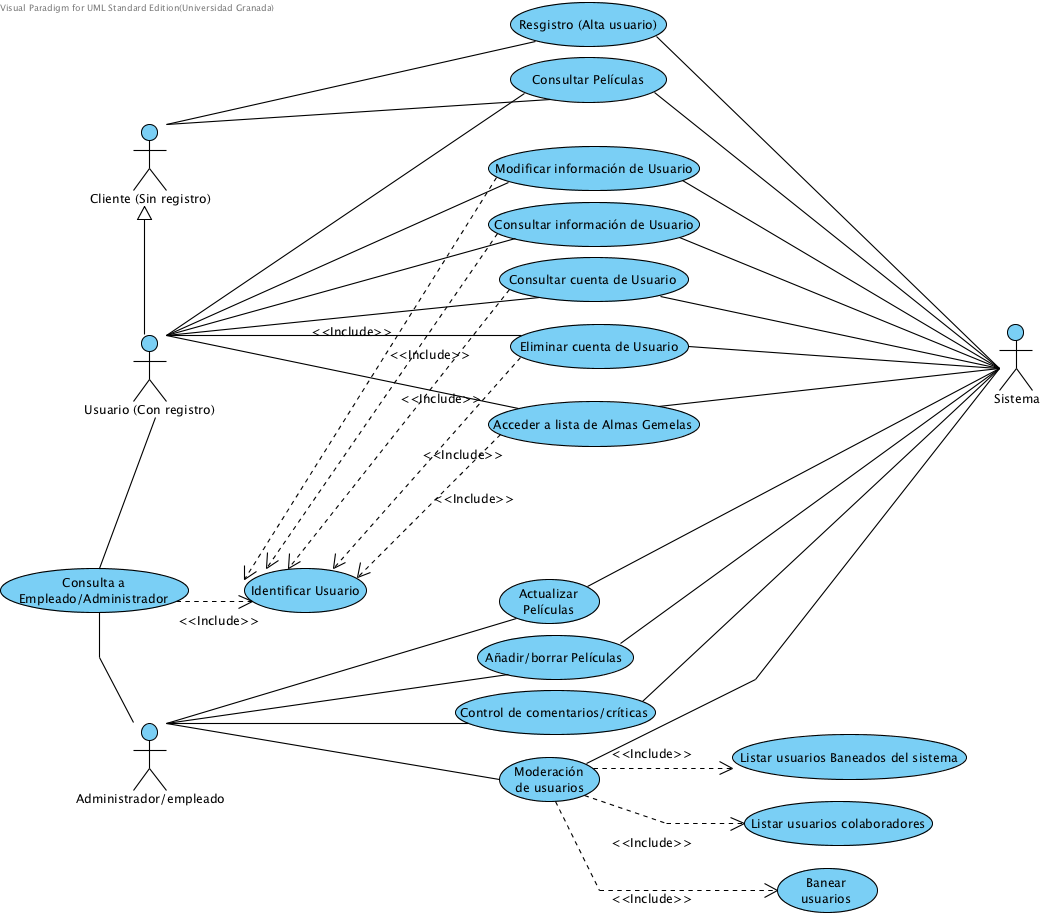
\includegraphics[scale=0.55]{GestiondeUsuarios.png}
   	\end{center}
\section{Descripción básica de casos de uso}


%======================================
%Ejemplo de tabla de casos de uso:
%======================================
\begin{table}[h]
\begin{tabular}{|l|l|l|l|l|l|}
\hline
\multicolumn{2}{|p{2cm}|}{Casos de uso}  & \multicolumn{3}{p{7cm}|}{} & CU-x \\
\hline
\multicolumn{2}{|p{2cm}|}{Actores}       & \multicolumn{4}{p{8cm}|}{}        \\
\hline
\multicolumn{2}{|p{2cm}|}{Tipo}          & \multicolumn{4}{p{8cm}|}{}        \\
\hline
\multicolumn{2}{|p{2cm}|}{Precondición}  & \multicolumn{4}{p{8cm}|}{}        \\
\hline
\multicolumn{2}{|p{2cm}|}{Postcondición} & \multicolumn{4}{p{8cm}|}{}        \\
\hline
\multicolumn{6}{|p{10cm}|}{Proposito}                                   \\
\hline
\multicolumn{6}{|p{10cm}|}{}                                            \\
\hline
\multicolumn{6}{|p{10cm}|}{Descripción}                                 \\
\hline
\multicolumn{6}{|p{10cm}|}{}                                            \\
\hline
Autor              &              & Fecha    &     &   Versión  &\\     
\hline
\end{tabular}
\end{table}


\end{document}
